\chapter[Understanding and Monitoring Untrusted Code]{Understanding and Monitoring Untrusted Code\footnote{The contents of this chapter is based on the paper: Understanding and Monitoring Embedded Web Scripts~\cite{FireInspector}.}}
\label{sec:fireinspector}

In Chapter~\ref{sec:esorics} we presented how fine-grained DOM access control can be achieved by modifying the Chromium browser, and a proxy-based automatic policy generator that infers private information based on differences of two responses.  While this is a solid first step, we think there are several issues with the design of the policy language and generator that may affect the usability of the tool.

First, the policy generator yields plenty of false positives on complex sites that include lots of dynamic content.  Because the content served each time could be different even in the same session, according to the design the policy generator will deem these differences as private content and thus over-restrict the third-party scripts.

Second, our previous solution does not offer site administrators a way to inspect and understand what is going on under the hood for third-party scripts.  Since the policy generator is likely to produce false positives (marking public content as private), admins will likely need to use a trial-and-error approach to make sure the strict policies do not break the scripts.  This process not only is tedious but may also expose more information than necessary for the scripts to work.  As add-on attributes to individual DOM nodes, the access control policies are hard to edit and maintain, especially across the entire website which may be consisted of many pages.  

Additionally, the proxy-based policy generator will not work very well in practice due to the duplicated traffic overhead and unwanted server-side state change.  To comply with the policy generator, a website will have to ensure no unauthenticated requests can make any changes to server state, which is often not the case nowadays.  This drawback will likely be the most important resistance to the deployment of our previous approach.

To avoid these issues, we now present an alternative design of a chain of server-side tools to assist developers to understand and monitor the third-party JavaScripts behavior.  Accesses to critical resources and policies for third-party scripts can be visually presented to the site administrators.  The visualization together with intelligible CSS/XPath selectors used in policy entries make them much easier to edit and maintain across the site.

\begin{figure}[tbh]
\centering
\includegraphics[width=0.8\textwidth]{figures/chapter6/overview}
\caption{Overview}
\label{fig:stOverview}
\end{figure}

Figure~\ref{fig:stOverview} gives an overview of our tool chain.  The rest of this chapter is organized as follows to describe each component separately: we first discuss the new policy language design that offers better flexibility and maintainability in Chapter~\ref{sec:policy}.  Then, we present our implementation of \st in Chapter~\ref{sec:st}, a modified version of the Firefox browser that is capable of intercepting and recording API calls from third-party scripts to critical resources, including the DOM, local storage, and network.  Chapter~\ref{sec:visualization} describes the \vis, a Firefox extension that uses the instrumented DOM maintained by \st to highlight nodes accessed by third-party scripts and help a site administrator understand script behaviors.  Chapter~\ref{sec:visualizationStories} describes some interesting findings we discovered using the \vis.  In Chapter~\ref{sec:pg} and~\ref{sec:sspolicies} we present some base policy examples, and then explain the new \pg tool which is used to automatically generate site-specific policies for site administrators.  We evaluate the effectiveness of \pg and how the entire tool chain performs under an anomaly detection deployment scenario in Chapter~\ref{sec:robustness}.  Finally, we conclude with related works (Chapter~\ref{sec:stRelatedWorks}) and deployment scenarios (Chapter~\ref{sec:stDeployment}) of the system.

\section{Policies}
\label{sec:policy}

A policy used in \st is a set of permissions that describe the permissible
behaviors for a script.  Our goal is to develop policies that are
precise enough to limit the behavior of a script to provide a desired
level of privacy and security, without needing to generate custom
policies for each page on a site.  Further, as much as possible, we want
to be able to reuse a script policy across all sites embedding that
script.  The challenge is the way a script behaves depends on the
containing page and how the script is embedded, especially in the
specific DOM nodes it accesses.  Our solution to this aims to make the
right tradeoffs between over-generalizing policies and requiring
page-specific policies, which we believe would place an unreasonable
burden on site administrators.

Policies are described by the following grammar:

\begin{grammar}\raggedright
<Policy> ::= <Permission>*

<Permission> ::= [<NodeDescriptor>:]<Action>[:<Param>*]

<Action> ::= <LocalStorage> | <BrowserConfiguration> | <NetworkRequest> | <DOMAPI> 

\end{grammar}

\noindent
We explain different types of actions in Section~\ref{sec:resources} and
node descriptors in Section~\ref{sec:DOMNodeDescriptor}.
Section~\ref{sec:interference} addresses the problem of interference
between permissions.

\subsection{Resources}\label{sec:resources}

The main resource accessible to scripts is the web page content,
represented by the Document Object Model (DOM) in the browser.  DOM
access includes all reads and modifications to the DOM tree, including
node insertion and removal, reading its \code{innerHTML}, and setting or
getting attributes.  For DOM permissions, the
\emph{Action} is the DOM API itself (e.g., \code{appendChild}) and
the \emph{NodeDescriptor} (see Section~\ref{sec:DOMNodeDescriptor})
specifies the set of nodes on which the action is allowed.  The \emph{NodeDescriptor} can be omitted to allow an API to be called on any DOM node.  The argument restriction is also optional as some APIs may be called without any argument.
Arguments are represented as regular expressions that match strings or
nodes.  A node used in an argument is matched by
its \code{outerHTML}.  In certain scenarios, the site owner may need to
make sure the node in the argument is a node that was created by a third-party script
(e.g., a node created by an advertising script to display ad content).  To enable this restriction, the
\code{[o]} (stands for `owned') tag may be inserted before the argument.  For example,
\policy{//DIV:RemoveChild:[o]<img src=`pic.jpg'>} allows the third-party script to remove an image, with the restriction that the image element must have been created by a script hosted by that same party (not from the original host).

In addition to the DOM, scripts have access to other critical resources.
These accesses are only allowed if a permission allowing the
corresponding \emph{Action} is included in the policy.  These
permissions do not include \emph{NodeDescriptor}s, since they are not
associated with particular DOM nodes.

\shortsection{Local storage} Accesses to \code{document.cookie} require
the \code{getCookie} or \code{setCookie} permission, while all other
accesses to local storage APIs (such as the \code{localStorage}
associative array and \emph{indexedDB}) require the \code{localStorage}
permission.

\shortsection{Browser configuration} Third-party scripts may access
user-identifying browser configuration, possibly to serve
customized scripts to different user groups.  However, such information can also be used to fingerprint
browsers~\cite{FPDetective} and identify vulnerable targets.  \st ensures all accesses to
these objects require corresponding permissions.  For example, the
\code{navigator.userAgent} action permission allows a script to obtain
the name and version of the client browser.

\shortsection{Network} Ensuring third-party scripts only communicate
with intended domains is critical for limiting information leakage.  A
script can initiate a network request many ways, including calling
\code{document.write} or related DOM insertion APIs, setting the
\emph{src} attribute of a \emph{img} node, submitting a form with a
carefully crafted \emph{action} attribute, or sending an explicit
asynchronous JavaScript request (AJAX).  Regardless of the method used
to access the network, transmissions are only allowed if the policy
includes the network permission with a matching domain.

\subsection{Node descriptors}
\label{sec:DOMNodeDescriptor}

A node descriptor is an optional matching mode (introduced later in this section)
followed by a node representation:

\begin{grammar}
<NodeDescriptor> ::= [<MatchingMode>:] <NodeSelector>

<NodeSelector> ::= <AbsoluteXPath> | <SelectorXPath> | <RegexpXPath> 
                   | {\bf \textasciicircum} <NodeSelector>

<MatchingMode:> ::= {\bf sub} | {\bf root}
\end{grammar}

\shortsection{Absolute XPaths} A DOM node can be specified using an
absolute XPath.  For example, \policy{/HTML[1]/BODY[1]/DIV[1]/} is an
absolute XPath that specifies the first DIV child of the BODY element of
the page.  Absolute XPaths are often useful for matching generic invisible
tracking pixels injected by third-party scripts.

\shortsection{Attribute-Based selectors} Nodes can also be specified
using Selector XPaths.  For example, \policy{//DIV[@class=`ad']}
specifies the set of all DIVs that have the class name \code{ad}.  This
permission is often used to capture the placeholder node under which the
third-party scripts should inject the advertisements.  Using a selector
may compromise security in that there might be other nodes on the
webpage that can be accidentally matched using the same selector.
Therefore, care has to be taken to make the selectors as restrictive as
possible to avoid matching unintended elements.  We discuss how the \pg
can assist administrators to achieve this goal in
Section~\ref{sec:policyGen}.  Another concern is that a third-party
script may modify the node attribute to make that node match the
selector on purpose.  To prevent this, the policy must not allow calls
to modify the attributes used in selectors (see
Section~\ref{sec:interference}).

\shortsection{Regular expressions} To offer more robustness and
flexibility, our node selector supports regular expressions in
XPaths.\footnote{XPaths that accept regular expressions have been
  proposed for XPath 3.0, but are not yet supported by any major browser.}
We found this necessary since many sites introduce randomness in page structure and node attributes.  For example, we found
that websites may embed an advertisement by defining its placeholder
DIV's ID as a string that starts with ``\code{adSize-}'', followed by the size of the ad (e.g. 300x250).  We use this
descriptor to specify these nodes:
\policy{//DIV[@ID=`adSize-\d*x\d*']}.

\shortsection{Contextual selectors} A node may be described by another
selected node's parent.  This is especially convenient when the accessed
node does not have any identifying attribute, but one of its children
does.  We support this by allowing a caret (\policy{^}) to be added
before a node selector to indicate how many levels to walk up the tree
when looking for a match.  For example, \policy{^^//DIV[@ID=`adPos']}
specifics the node two levels above the DIV element whose id is
\code{adPos}.

Similar to the parental context, a node can be described as another
selected node's child node.  For example,
\policy{//DIV[@ID=`adPos']/DIV[2]} specifies the second DIV child of the
DIV element whose id is \code{adPos}.

\shortsection{Matching mode} Many site-specific DOM accesses happen as a
result of advertising and widget scripts injecting content into the
page.  These scripts often follow similar access patterns, and we define
two matching modes that can be used to adjust matching.  When no mode is
provided, only nodes specified by the given node representation match.

The \emph{subtree} matching mode matches all children of nodes that are
matched by the node selector.  For example,
\policy{sub://DIV[@id=`adPos']} selects all children of the DIV element
whose id is \code{adPos}.  This matching mode is particularly useful for
scripts such as advertising and social widgets that add content into the
page.  They often touch all children of the placeholder node.  However,
the node structure inside the injected node may be different between
requests, making it hard to describe using the strict-matching mode.  In
this scenario, a policy that limits script access to a subtree is
more plausible.

\emph{Root mode} covers all nodes that are ancestors to the selected node.  For example,
\policy{root://DIV[@id=`adPos']}
describes all ancestor nodes of the DIV element whose id is \code{adPos}.  

\begin{algorithm}[bth]
  \floatname{algorithm}{Listing}
  \caption{Script access pattern example}
  \label{listing:RootModelEvidence}
  \begin{algorithmic}[1]
		\Statex \hspace{-15pt} /BODY[1]/DIV[3]/DIV[4]/DIV[1]:AppendChild:...\par
		\Statex \hspace{-15pt} /BODY[1]/DIV[3]/DIV[4]:GetClientWidth\par
		\Statex \hspace{-15pt} /BODY[1]/DIV[3]:GetClientWidth\par
		\Statex \hspace{-15pt} /BODY[1]:GetClientWidth\par
  \end{algorithmic}
\end{algorithm}

We use a commonly seen advertising script access pattern, shown in
Listing~\ref{listing:RootModelEvidence}, to explain why this is useful.
In this example, the actual meaningful operation is done on the node
described in the first line, but the script accesses all of its
ancestor nodes.  The APIs called on these nodes usually do not reveal
much information, e.g. \code{GetID} or \code{GetClientWidth}.  We suspect this is due to the script using a
JavaScript library helper such as \emph{jQuery}.  To capture this
behavior pattern, the root matching mode can be used to match all three
accesses to \code{GetClientWidth} in Listing~\ref{listing:RootModelEvidence}, as shown here:

  \begin{algorithmic}[1]
		\Statex \policy{/BODY[1]/DIV[3]/DIV[4]/DIV[1]:AppendChild}\par
		\Statex \policy{root:/BODY[1]/DIV[3]/DIV[4]/DIV[1]:GetClientWidth}\par
  \end{algorithmic}

\subsection{Permission interference}\label{sec:interference}

Attribute-based selectors open the possibility that one permission
interferes with another, undesirably extending the collection of matched
nodes and allowed APIs.  For example, suppose the following two
permissions were granted:

  \begin{algorithmic}[1]
		\Statex \policy{//DIV[@class=`tracker']:SetId}\par
		\Statex \policy{//DIV[@id=`adPos']:AppendChild}\par
  \end{algorithmic}

The first permission allows the \emph{id} attribute to be set on any
DIV node that has a certain \emph{class}; the second allows
\code{appendChild} to be called on any DIV node that has a
certain \emph{id}.  In combination, they allow the script to set
\emph{id} attribute of any DIV that has class \code{tracker},
thus gaining permission to call \code{appendChild} on those
nodes.

Manually-created policies need to be carefully examined to exclude the
use of certain attributes as selectors if policies from the same third
party allows them to be set freely.  The \pg tool is designed to
automatically avoid such conflicts (Section~\ref{sec:policyGen}).

Sometimes the site owner wants to grant third-party scripts permission
to call any API on certain nodes (e.g., placeholder nodes to be replaced
by ads or widgets).  However, enabling a wild card action that matches
all DOM APIs is dangerous due to possible interference scenarios.  To
support this scenario, we created a special action denoted by the
exclamation mark to indicate all API calls except those that may cause
policy interferences.  

For example, the permission, \policy{//DIV[@class=`content']:!}, allows the script to
call any API on any DIV node with class \code{content}, except ones that
may set the class attribute to prevent self-interference.  Similarly,
the permission, \policy{//DIV[@id=`adPos']:!}, allows any API on the
DIV with id \code{adPos}, except for ones that may set its id attribute.
However, when these two permissions co-exist for a script, they will
forbid API calls to both \code{setClass} and \code{setID}, to prevent self and mutual
interference.  This feature proved to be extremely helpful in our
evaluation (Section~\ref{sec:usingPG}).

\section{Inspecting Script Behavior}
\label{sec:st}

\st\ is a tool for inspecting the behavior of scripts, focused on
monitoring how they manipulate resources and detecting violations of the
permissions we defined in Section~\ref{sec:policy}.  Next, we explain
how \st\ records third-party script
behavior. Section~\ref{sec:checkingPolicy} discusses how the records are
checked against policies or output to logs for admin's inspection.

\subsection{Recording accesses}
\label{sec:recording}

\st is implemented by modifying Firefox to add hooks to JavaScript API calls.  \st records all API calls made by scripts that involve any of the critical resources mentioned in Section~\ref{sec:resources}.  Modifications are primarily made in the DOM-JS binding section, and approximately 2000 lines of code were added.  The modified browser retains the same functionality as a normal browser, with the addition of access recording capability.

\shortsection{DOM access recording} We modified Firefox's C++ implementations of relevant DOM APIs such as
\code{insertBefore}, \code{setAttribute} and \code{document.write} to record DOM accesses.
Complete mediation is ensured as Firefox uses a code generator to
generate the C++ implementation according to the defined interfaces, and
our modifications are inserted to the code generator, rather than
individual implementations.

\st augments each DOM node with a hidden field to record accesses to
that node.  For each access, the caller identity as well as the API name
and optional arguments are recorded in this hidden field.  Thus,
function call information is preserved with the node for the node's
lifetime.  We discuss necessary steps to address node removal events in
Section~\ref{sec:checkingPolicy}.

\shortsection{Recording other actions}  For non-DOM resources, we also add hooks to their C++ implementations. Since these calls are not tied to a particular node, the caller records are stored in the hidden field on the \code{document} object of the page. 

\shortsection{Script-injected nodes}
To support the \code{[o]} tag (Section~\ref{sec:resources}),
\st tracks the \emph{ownership} of a node by augmenting node-creation
APIs such as \code{document.write} and \code{document.createElement}.  If a
third-party script creates a node and inserts it into the document, we
record the responsible party as that node's owner.  This feature is especially useful since the host can simply ignore
accesses to third-party owned nodes and ensure its own nodes are not used in any arguments.

\shortsection{Attribution}\label{sec:attribution}
Correctly attributing actions to scripts is important, since policies
are applied based on the domain hosting the script.  To obtain the
identity of the caller, \st leverages existing error handling mechanisms
implemented in Firefox.  Firefox's JavaScript engine, SpiderMonkey,
provides a convenient API to obtain the current call stack.  It contains information about the script's origin and line
number, which are all we need to attribute the accesses.  Additionally, a site administrator can provide \st with a list of whitelist domains.  When a call takes place, \st records all third party domains on the stack, except for host domain and whitelisted domains.

The call stack information is sufficient to correctly attribute most
introduced dynamic inline code (e.g., through \code{eval} or \code{document.write}), but falls short when
an inline event handler is registered to an object and is later
triggered.  \st currently cannot handle this scenario and we rely on
future Mozilla patches to fix this issue.

\subsection{Checking policies}\label{sec:checkingPolicy}

To check recorded accesses against a given policy, \st introduces the \code{checkPolicy} function.  When this function is called, \st walks the DOM tree, collects all DOM accesses and other accesses stored in the document node, and checks them against the policy.  The violating accesses can be used for visualization by the \vis (Section~\ref{sec:visualization}) or as input to \pg\ to use in automatic policy generation (Section~\ref{sec:pg}).  A log file is also produces for site administrators to inspect manually (an example log file with violations serialized to absolute XPaths is shown in Listing~\ref{listing:RootModelEvidence}).  

As opposed to the straightforward design of recording and serializing violations as the accesses happen, our design only records them at access time, but collects and serializes the access records when the page unloads.  The additional complexity here may be counter-intuitive; however, such a delay is important for improving the robustness of DOM permissions.  For example, a third-party script may obtain the height of a node before the host script sets its id to `adPos'.  In this case, the permission \policy{//DIV[@id=`adPos']:GetHeight} cannot cover this access if the policy is checked immediately, since its id is yet to be set to `adPos'.  Due to the nondeterministic execution order of scripts, checking policy when the access happens is not a good choice.

However, this leaves opportunities to evade mediation if a script reads content of a node and later removes that node.  To eliminate this leak, we tweak the APIs that directly (e.g. \code{removeChild}) or implicitly (e.g. \code{setInnerHTML}) remove DOM nodes: \st automatically performs \code{checkPolicy} on the to-be-removed nodes and stores the violations into the hidden field of its owner document before they are actually removed.

\section{Visualization}
\label{sec:visualization}

To visualize the access violations and permission candidates, we built
\vis, a \st extension that takes the instrumented DOM and accesses as
input, offers a convenient user interface (shown in
Figure~\ref{fig:visualizerScreenshot}) to display the page content that
is read or modified by the third party.  We envision \vis being used by
concerned site administrators who hope to gain insight as to how the
embedded scripts interact their websites.  With this goal in mind, we
next describe using \vis from the perspective of a site administrator
seeking to understand the behaviors of scripts on her site.  We present
some interesting discoveries from our experiments visualizing script
behaviors in Section~\ref{sec:visualizationStories}.  The \vis may also
be used to visualize the node collections that are matched by a
permission.  This can be used together with the \pg to help
administrators make their decisions (see Section~\ref{sec:policyGen}).

Figure~\ref{fig:visualizerScreenshot} is a screenshot of visualized accesses at \url{foxnews.com}.  The left sidebar displays the domains of all 
third-party scripts embedded on the page (\url{googleadservices.com} and
\url{googlesyndication.com} shown in the screenshot), and the site administrator
may click a domain (\url{googlesyndication.com} in this
example) to expand it and highlight the nodes access by scripts from that domain.

\begin{figure}[!b]
\centering
\includegraphics[width=0.47\textwidth]{figures/chapter6/visualizerScreenshot}
\caption{Visualizer interface}
\label{fig:visualizerScreenshot}
\end{figure}

\vis classifies DOM accesses into three subcategories --- \emph{getContentRecords} (reading the content of a node,
e.g. \code{getInnerHTML}), \emph{setterRecords} (modifying the attribute or
content of the node), and \emph{getterRecords} (reading properties of a node
other than the content itself).  These categories help administrators quickly locate the accesses of interest.  Uses may click on these categories to further expand them into individual accesses.

Users may hover over each entry to highlight the
accessed node on the right side.  They may also click on a category
to see all nodes that were accessed that way (enclosed by double blue border and covered in a faint blue overlay in the screenshot).
For accesses to nodes that any third-party \emph{owns} (See Section~\ref{sec:resources}), the entry is displayed in green and enclosed by a dashed border.  In Figure~\ref{fig:visualizerScreenshot}, the scripts form \url{googlesyndication.com}, representing one of Google Ad networks,
accessed non-content properties of its own inserted ads on
\url{foxnews.com}.  Upon seeing this, the administrator may proceed to make
decisions to approve embedding Google Ads on their site.

\section{Findings}
\label{sec:visualizationStories}

We used \st and \vis to examine the top 200-ranked US websites from
\url{Alexa.com}.  Assuming the role as their administrators, we aim to
understand how resources are accessed by embedded scripts.  We created accounts at these sites and logged into them if possible.  We also attempted some typical user actions on these sites, such as adding merchandise into cart for e-commerce websites, and visiting user profile pages for sites that support login.

\shortsection{Browser Properties} Almost all of the tested third-party
scripts access a number of generic properties of the browser including
the \code{navigator}, \code{screen} object, and some properties of root
DOM nodes such as the \emph{document} and \emph{body} element.  Although
this information information could also be used for fingerprinting
browsers~\cite{FPDetective}, we consider this behavior reasonable for
most scripts since they determine what content to serve based on the
browser's vendor and version (\code{navigator.userAgent}), and user's
screen size (\code{screen.height} or \code{body.clientHeight}).

\shortsection{Network} Another unsurprising but concerning fact is that
most scripts we observed send out network requests, at least to their
own host servers.  Quite a few advertising scripts (e.g.,
\url{googleadservices.com}, \url{moatads.com}) also send requests to
many other destinations (mostly affiliate networks).

\shortsection{Modifying page contents} Advertising scripts and social
widget scripts often modify the container page by injecting or replacing
placeholders with content in the page, as seen in
Figure~\ref{fig:visualizerScreenshot}.  In addition, multiple tracking
scripts insert tracking pixels and scripts from other tracking
companies, and advertising scripts may inject other scripts from
affiliate programs.  However, it is hard for us to determine if such
modifications violate the site administrator's expectations.

\shortsection{Reading page content} Finding scripts that read specific
page content was less common, but we did observe this for several
scripts.  The content read ranges from a specific element to the full
document.  Reading page content may compromise user privacy.  \vis
alerts the site administrators to scripts that read page content by
presenting them in a different category, especially when network access
also happens in the same session.

Scripts from \url{adroll.com} read the DOM element that displays the SKU
number of online merchandises on certain e-commerce pages.  We initially
discovered this when using \vis on \url{newegg.com}, but later found
similar behaviors on \url{dx.com} and \url{bhphotovideo.com}.  We manually examined \url{Adroll}'s script after using
deobfuscation and code beautifiers, and found out that it indeed
contains case-switch statements to handle many particular e-commerce site
layouts.

According to \emph{Adroll}'s company website, the script is used for
ad-``retargeting'' purposes.  This means the company learns the user's
purchasing interests from shopping sites that embed the script, and then
displays relevant advertisements to the user on other sites, hoping for
a better conversion rate.  It seems likely that in this case Newegg
agreed to embed the \url{adroll.com} scripts, however, its users have no
idea their detailed interactions with \url{newegg.com} are being tracked
by an external service.  Newegg's privacy policy states vaguely that it
may employ third-party companies to perform functions on their behalf
and the third parties have limited access to user's personal
information, but nothing that suggests user's shopping actions are
immediately revealed to third parties.

\begin{figure}[tbh]
\centering
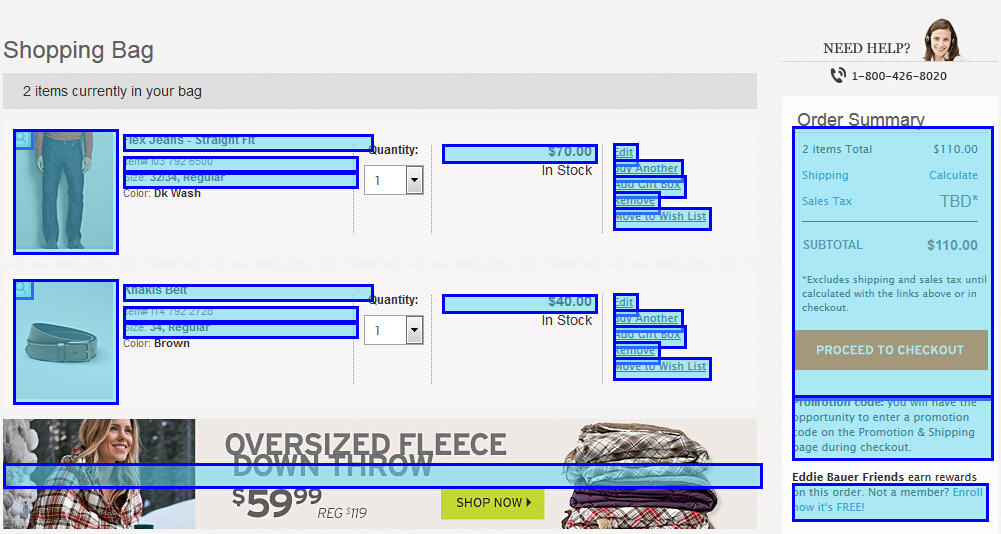
\includegraphics[width=0.47\textwidth]{figures/chapter6/EddieBauerCart}
\caption{Script reading EddieBauer's shopping cart}
\label{fig:EddieBauerCart}
\end{figure}

\begin{figure}[tbh]
\centering
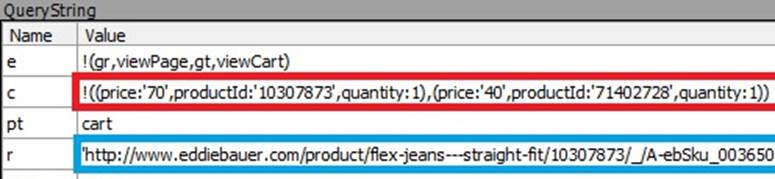
\includegraphics[width=0.47\textwidth]{figures/chapter6/EddieBauerRequest}
\caption{Script sending out EddieBauer's shopping cart information}
\label{fig:EddieBauerRequest}
\end{figure}

Similar behaviors were observed on other e-commerce sites (e.g.,
\url{autozone.com}, \url{eddiebauer.com}) involving other third-party
service providers (e.g., \url{monetate.com}, \url{certona.com},
\url{tiqcdn.com}).  For example, a script from \url{monetate.com} that
is embedded by EddieBauer's site accesses and transmits user's shopping
cart information (Figure~\ref{fig:EddieBauerCart}).
Figure~\ref{fig:EddieBauerRequest} shows a captured form submission
request in Fiddler~\cite{Fiddler} that was initiated by a script from
\url{monetate.com}, with red box highlighting the cart information, and
blue box highlighting the product page.

In another case, \url{crwdctnrl.net} scripts read user inputs on some
sites.  On \url{ask.com}, the script reads the main text input box used
by users to submit questions.  On \url{weather.com}, it reads the text
input in which the user enters their zip code or address to request
local weather.  The script subsequently sends traffic back to its own
server, although we are not able to confirm that the traffic leaks the
user input.

Many scripts occasionally read certain properties from a particular node
type, for example, \url{scorecardresearch.com} scripts read all images'
\code{outerHTML} on \url{allrecipes.com}.  Since \url{allrecipes.com}'s
user login information is included as an attribute of user's login
avatar, comScore (the company who operates \url{scorecardresearch.com})
may obtain user's information through the image accesses.  Other
commonly accessed tag/attribute pairs include getting the \emph{href}
attribute of all \emph{a} elements or the \emph{content} attribute of
all \emph{meta} elements.  Either of these may contain sensitive
information.

The most concerning scenario comes from the sites that embed
\url{krxd.net} scripts, which \emph{consistently} read \emph{all}
content of the embedding host page.  This includes all values of all
text nodes, and \code{innerHTML} of all elements.  We have also observed
that scripts from this domain send requests to at least 25 different
domains, requesting additional scripts and tracking pixels.  We find
this behavior appalling, and cannot fathom the reasons behind it by
looking at its description on Krux's company website.

\section{Developing Base Policies}
\label{sec:pg}

The base policy for each script is a policy intended to be used across
all sites that embed that script.  Obtaining a script's base policy only
requires a one-time effort, with perhaps additional work required to
update the policy when the script is modified significantly.  Hence, it
is not necessary to automate developing base policies.  In deployment,
the base policies could be centrally maintained and distributed, either
by the script's service provider (perhaps motivated to disclose its
behavior to earn the trust of potential integrators), or by a trusted
security service.

In this section, we report on our experience using the logs generated by
\st to develop base policies for 25 popular third-party scripts.  The
\pg and \vis are often not needed to develop base policies (especially
for the script's author who should already understand its expected
behavior), as the base policy often does not contain specific DOM
accesses.

\subsection{Evaluation method} 
\label{sec:evalApproach}

We manually developed policies for 25 selected scripts.  The manual
effort required to develop these policies limits the number of scripts
we can examine.  However, the scripts we examined are the most popular
ones among their respective categories, and our experience from
Section~\ref{sec:visualizationStories} indicates that their behavior is
a good representation of extant third-party scripts.

\renewcommand*{\UrlFont}{\ttfamily\smaller\relax}

To select the 25 scripts, we first took the 1000 highest-ranked websites
from \url{alexa.com} and visited their homepages repeatedly over a week,
crawling pages to collect embedded scripts.  We extracted all
third-party scripts seen in this process, and sorted them based on the
number of occurrences.  We took the top 25 on the list and manually
visited 100 sites which embed each script, sampled randomly from the 1000 sites on the \url{alexa.com} list.\footnote{In selecting the container sites, we excluded
  inappropriate sites including those which the embedded scripts do not
  access anything, trivial sites that have few subpages and content,
  sites with objectionable content (e.g., porn), and foreign language
  sites for which we were unable to register and login.  The full list is available at \renewcommand*{\UrlFont}{\smaller\tt\relax}\url{ScriptInspector.org/sites}.}

\renewcommand*{\UrlFont}{\normalsize\tt\relax}

Of those 100 sites, 77 include user registration and login
functionality.  For each of these, we manually created a test account
and logged in to the website to mimic a typical user's experience.
After user sessions are prepared, we first visit each site's homepage,
follow links to navigate to several subpages, and call
\code{document.checkPolicy} to output an access report.  We repeat this
process until no new accesses are seen in five consecutive requests.  We
then manually extract the most commonly observed accesses to form the base
policy.  Our overall goal in writing base policies is to allow all
behaviors that an integrator is likely to encounter without
over-generalizing.  The base policy should contain mostly special API
accesses and generic DOM accesses to the root elements of the page
(\emph{document}, \emph{body} and \emph{head}).  However, if certain DOM
accesses with fixed patterns are seen consistently, they are also
included in the base policy.

\subsection{Base policy examples}  

For clearer presentation, we discuss base policies organized by grouping
scripts into four categories: \emph{analytics}, \emph{advertising},
\emph{social widgets}, and \emph{web development}.

\shortsection{Analytics} Analytics scripts are typically transparent to
the site visitors and do not affect the functionality or visual
output of the embedding webpage.  Their base policies include a fixed
group of sensitive APIs such as setting and reading
\code{document.cookie}, but not any specific DOM accesses.

\begin{algorithm}[bt]
	\setcounter{algorithm}{0}
  \floatname{algorithm}{Policy}
  \caption{Google Analytics Base Policy}
  \label{policy:gaPolicy}\small\raggedright
  \policy{/HTML[1]/BODY[1]:GetId}; \policy{/HTML[1]/BODY[1]:ClientHeight}; \policy{/HTML[1]/BODY[1]:ClientWidth};
  \policy{/HTML[1]:ClientHeight}; \policy{/HTML[1]:ClientWidth}; \\
  \vspace*{1ex}
  \policy{navigator.javaEnabled}, \policy{navigator.language}, \policy{navigator.plugins}; \policy{navigator.cookieEnabled}; \policy{navigator.userAgent};
  \policy{screen.height}; \policy{screen.width}; \policy{screen.colorDepth} \\ 
  \policy{GetCookie}; \policy{SetCookie} \\
  \vspace*{1ex}
  \policy{NetworkSend:doubleclick.net}; \policy{NetworkSend:google.com}; \policy{NetworkSend:google-analytics.com} \\
  \vspace*{1ex}
  \policy{/HTML[1]/HEAD[1]>InsertBefore:\[o\]}\\
  \hspace*{2em}\policy{<script[^<>]*></script>}
\end{algorithm}

As the most frequently embedded script by far, Google Analytics exhibits
a very stable behavior pattern described by
Policy~\ref{policy:gaPolicy}.  Other than the final permission, all its
accesses can be categorized into three categories: 1) Generic DOM
access: reading the size of the \emph{body} element; 2) special property
access: testing the browser's configuration, reading and writing
cookies; and 3) network access: sending information back to Google
Analytics servers via setting the \code{src} property of an image
element.  This reassures the site owner that the Google analytics script
is not accessing site-specific information or making content changes to
the site.  The final permission is needed because the Google Analytics
script inserts dynamically-loaded scripts into the page.  The
\policy{\[o\]} limits the insertions to nodes owned by the script.  The
parameter is a regular expression that specifies the element type
inserted must be a script.  Note that the network policies still apply,
restricting the domain hosting the dynamically-loaded script.  Also,
recall that this same base policy still applies to any scripts from the
same domain due to our access attribution implementation, so dynamically
loading scripts does not provide extra capabilities.

Another popular embedded script, Quantcast analytics, exhibits similar
behavior with the addition of reading the \emph{content} attribute of
all \emph{meta} elements.  Common practice suggests using these
attributes to mark keywords for the document, so Quantcast is likely
collecting these keywords.  In sites that embed Chartbeat analytics, the
\emph{src} attributes of all \emph{script} elements on the page are read
by Chartbeat, along with \emph{href} and \emph{rel} attributes of
\emph{link} elements.  This is a somewhat surprising, yet common
behavior that was also observed for several other scripts.  Chartbeat also
maintains a heartbeat message protocol with the backend server and
multiple request-response pairs are observed per session.

All the major analytics scripts appear to have sufficiently limited
behaviors that containing sites will not need site-specific policies.
Base policies can cover all observed behaviors without including any
permissions that allow access to ob\-vi\-ous\-ly sensitive resources and
content-changing APIs.

\shortsection{Advertisements} Google offers the most widely used
advertising service through AdSense and DoubleClick.
Policy~\ref{policy:GoogleAdsense} is an excerpt of the policy for
\url{googleadservices.com}, whose behaviors are representative of most
advertising scripts.

The AdSense script accesses several browser properties similar to the
analytics scripts, but also injects advertisements into the page and
often inserts a hidden empty frame or tiny image pixel for bootstrapping
or tracking purposes.  The tracking pixels are always injected into the
\emph{body} or \emph{document} element, and the last
permission in Policy~\ref{policy:GoogleAdsense} allows such
behavior.

The node where the actual advertisements are injected, however, varies
from site to site.  As a result, the base policy only covers the most
popular use, described by the \policy{//DIV[@id=`div-gpt-ad-.*']:!}
permission. This allows any APIs to be called on a node whose id starts
with \emph{div-gpt-ad-}, except those that may modify attribute names in node
descriptors of itself and any other permissions that belong to the same script.  Behaviors of other ways of integrating AdSense need to be covered by site-specific policies
(Section~\ref{sec:sspolicies}).

\begin{algorithm}[bt]
  \floatname{algorithm}{Policy}\raggedright
  \caption{Google Adsense Base Policy Excerpt}
  \label{policy:GoogleAdsense}\small\raggedright
\policy{//:GetAttribute:data-ad-container}; \policy{//:GetId} \\
\vspace*{1ex}
\policy{//DIV[@id=`div-gpt-ad-.*']:!} \\
\vspace*{1ex}
\policy{/HTML[1]/BODY[1]:document.write:}\\
\hspace*{2em}\policy{<img src=`googleadservices.com'/>} \\
\end{algorithm}

Scripts from \url{moatads.com}, \url{rubiconproject.com},
\url{adroll.com} and \url{adnxs.com} all exhibit similar behaviors to
Google advertising scripts.  In addition, the \url{moatads.com} scripts
occasionally read the \emph{src} attribute of all \emph{script} and
\emph{img} elements.  This behavior is dangerous and could result in
information leakage. Since it is observed on many containing sites,
however, we add it to the base policy despite the fact that it may only
happen once in many visits.  Scripts from \url{betrad.com} also access
localStorage APIs, presumably adding an extra tracking approach should
the user reject or delete their cookie.

Compared to analytics scripts, the advertising scripts exhibit behaviors
that vary substantially across sites. Hence, additional site-specific
permissions are often necessary to accurately describe their behavior.
The base policies for ad scripts also include more permissions, such as
reading attributes of all nodes with a certain tag name and appending ad
contents and tracking pixels to the \emph{body} element.

\shortsection{Social widgets} Social widget scripts behave similarly to
advertising scripts.  As an example, Policy~\ref{policy:TwitterPolicy}
shows the base policy for \url{twitter.com} scripts which includes
permissions for getting and setting twitter-specific attributes,
accessing content size, injecting content, and replacing placeholders of
the page.  As we see in Section~\ref{sec:sspolicies}, social widget
scripts often require site-specific policies.

\begin{algorithm}[bth]
  \floatname{algorithm}{Policy}
  \caption{Twitter Base Policy Excerpt}
  \label{policy:TwitterPolicy}\small\raggedright
\policy{//:GetAttribute:data-.*}; \policy{//:SetAttribute:data-twttr-.*}; \\
\policy{//:ReplaceChild:[o]}\\
\hspace{2em}\policy{<iframe data-twttr-rendered=`true'></iframe>}\\
\hspace{2em}\policy{<a class=`twitter-share-button'></a>} \\
\policy{sub:^//A[@class=`twitter-share-button']:GetAttribute:height}\\
\end{algorithm}

\shortsection{Web development}\label{sec:bpWebDev} Finally, we consider
web development scripts such as web A/B testing scripts from
\url{optimizely.com} and the jQuery library hosted on
\url{googleapis.com}.  Due to their broad purpose, the behavior of these
scripts differs significantly from those in the previous three
categories.  For example, the \url{optimizely.com} script modifies all
``comment'' buttons on \url{guardian.com}, inserts a style element on
\url{magento.com}, but did not access any part of the DOM on
\url{techcrunch.com}.  What these scripts do is depends a great deal on
how the site owners use them.

Effective base policies cannot be developed for these scripts --- their
behavior varies too much across sites and even across requests on the
same site.  Web developers using these scripts would need to develop a
custom policy for them, based on understanding what the script should do
given their intended use.


\section{Developing Site-Specific Policies}\label{sec:sspolicies}

Site-specific policies are needed for scripts that require different
permissions depending on how they are embedded. To aid site
administrators in developing appropriate site-specific policies, we
developed the \pg tool to partially automate the process.  The \pg
generates permission candidates based on violations to existing policies
reported by \st.  The site administrator can use \vis to examine the
candidate permissions and either select appropriate permissions to
include in the script's policy or decide not to embed the script if it
requires excessive access.  Section~\ref{sec:policyGen} introduces the
\pg tool and Section~\ref{sec:usingPG} reports on our experience using
it.

\subsection{\pg}\label{sec:policyGen}

With the base policies in place, the site-specific permissions typically
need to allow access to specific DOM elements such as placeholders for advertisements.
Our key observation behind the \pg is that although
absolute properties of these nodes vary across different pages and requests, good selector patterns can often be found that hold site-wide, due to consistencies within the web application design.  For example, the DOM
representations of the access nodes often have some common property such
as sharing a class which other elements on the same page do not have.

For example, consider these two CSS selectors describing advertisements observed on two requests to
\url{mtv.com}:
\begin{quote}
\policy{div#adPos300x250}\\
\policy{div#adPos728x90}
\end{quote}
These ad containers have different \emph{id}s, but their \emph{id} always starts with the string `adPos', followed by a pair
of height and width parameters.  Patterns like these are straightforward for site administrators to understand and can be inferred automatically from access reports.  

To use \pg, the user starts \st with the \pg extension.  \st is
configured to load base policies from a file to provide the initial base
policy for the scripts.  The user visits the page of interest, and then
clicks on the \pg extension button to start the process.  \pg generates
permission candidates, which are presented to the user using \vis.  The
user can then select permissions to add to the site-specific policy for
the script.  The user can continue visiting additional pages from the
site, invoking \pg, and refining policies based on automated
suggestions.

When the user invokes \pg, it obtains a list of violating records from
the instrumented DOM by calling \code{document.checkPolicy}.  It
initially generates a set of simple \emph{tag permission} candidates
which match DOM accesses only by their node name, API name, and
arguments, but not by attribute-value pairs.  This searches for simple
permissions like \policy{//DIV:getID}.  These candidates are selected by
counting the number of accesses to each node name and comparing it to
the total number of occurrences of that tag in the document.  If the
ratio reaches a threshold (customizable by the user; the default is 25\%
which we have found works well), a tag permission is proposed for that
API call.  Accesses that match this permission are removed from the set
of violating accesses for the next phase.

Finding good permission candidates that involve complex DOM selectors
is more challenging, but important to do well since these are the
permissions that would be hardest for a site administrator to derive
without assistance.  In Section~\ref{sec:visualizationStories}, we
observed that most accesses by a third-party script can be divided into
two categories: those that happen on ``nodes of interest'', and those
that can be covered by adding root, parent or sub prefix to the nodes of
interest.  The node of interest often has content modification APIs
called upon them (e.g., \code{appendChild}, \code{setInnerHTML}), or is
the deepest node accessed along the same path with other accessed nodes.
For example, the first node listed in
Listing~\ref{listing:RootModelEvidence} would be a node of interest
because it's the deepest node accessed.  

Following this observation, the next step is for \pg to develop a set of
selector patterns using attribute names for all nodes of interest,
excluding those that could interfere with current permissions (as
described in Section~\ref{sec:interference}).  Then, it produces an
attribute-value pair pattern candidates for each node of interest.  Our
implementation uses heuristics to synthesize four types of patterns for
each attribute name candidate: \emph{matches exactly}, \emph{matches
  all}, \emph{starts with}, and \emph{ends with}.  For the latter two
pattern types the generator calculates the strictest restriction without
sacrificing the number of accesses it matches, and then selects the best
pattern type that matches the most violations out of the four.  After a
best pattern and pattern type has been determined for each attribute
name, the generator sorts them by the number of matched violations of
each attribute name's best pattern, but excludes those which also
accidentally match any untouched nodes.

We provide an option to allow the generator to accept a pattern if it
matches some untouched nodes below a threshold ratio.  An example of
where this is useful occurs with advertising scripts that do not fill
not all advertisement spaces in one response, but instead leaves some
untouched for later use.  The decision regarding whether to accept
over-matched patterns is left to the developer, but it is important that
such patterns are clearly presented by \vis.
 
The best qualifying permission is then added to the set of permission
candidates that will be presented to the user, and all accesses matching
that permission are removed.  The process repeats until there are no
nodes of interest left.

If any violating accesses remain after all nodes of interest have been
removed, \pg examines if the remaining unmatched violations involve
either a parent, ancestor, or descendent of any node of interest.  If
so, a corresponding \policy{parent}, \policy{root}, or \policy{sub}
permission is proposed.

It is ultimately up to the developer's discretion to accept, reject, or
tweak the generated permissions.  To ease this process, the policy
candidates can be viewed using \vis.  The presentation is similar to
what is described in Section~\ref{sec:visualization}, and developers may
click on individual permissions to view the nodes they cover.

In the next section, we see that although the initial guessed
permissions are not always perfect, only minor tweaks are needed to
reach effective site-specific policies for most scripts and sites.  This
manual approval process is important for developing good policies, but
also valuable since our goal is not to produce policies that completely
describe the behaviors of all scripts on the site, but to help site
administrators identify scripts that are exhibiting undesirable
behaviors on their site.

\subsection{Adjusting permission candidates}\label{sec:usingPG}

We want to understand how much work is required to develop effective
site-specific policies for a typical website using our tools, assuming
base policies are provided for all scripts on the site.  In this
section, we describe manual efforts involved in using \pg on typical
sites and show some examples of site-specific policies. We defer the
discussion of quantitative results to Section~\ref{sec:robustness}.

To evaluate the \pg from a site administrator's point of view, we first
set up a crawler robot that visits a new set of 100 test sites using
\st.  The goal of the robot is to simulate regular users' browsing
actions to explore site-specific behavior of embedded scripts.  Given
the URL of a test site, the robot first visits that URL using the \st,
and waits for 30 seconds after the page has finished loading (or times
out after 60 seconds).  Then, it navigates to a randomly selected link
on the page whose target has the same domain as the test site.  We chose
not to navigate the robot away from each page right after it completes
loading because certain third-party scripts may not start to execute
after the page has loaded.  Upon page unloading, the robot calls
\code{document.checkPolicy} to log the violating traces.

The robot repeats the navigation until it has successfully navigated
five times for that test site, before moving on to the next.  If the
robot cannot find a link on the current page (or if the browser
crashes), it goes back to the homepage and resumes from there.  The scan
explores each site five levels deep to simulate user browsing behavior.
Finally, after the robot successfully navigated 5 times for all 100
sites, it restarts the whole process from the first site.

Whenever \st outputs a violation to existing policies on a site, further
visits to that site are postponed until we manually examine the violation using
\pg and add necessary permissions to the policy.  This is to prevent
similar violations being recorded multiple times.

We ran the evaluation from 28 December 2014 to 6 February 2015, a total
of 40 days.  For each site, the experiment contains two stages: an
initial stage to train a reasonably stable model, and a testing stage to
estimate how many violations would be reported if the policy were
deployed.  We initially define the training phase to last until after
\st completes 100 requests to that site without recording a single alarm
(we show how this threshold can be tuned in
Section~\ref{sec:robustnessResults}).

\shortsection{Permission adjustment examples} Depending on the
complexity of the site, generating and tweaking the policy for one site
may take from a few minutes up to half an hour based on our experience.
The cost varies due to factors such as the number and complexity of
scripts the site embeds, and how much pages differ across the site (for
example, in where they place advertisements).  The results here are
based on the first author's experience, who, as creator of \pg and \vis,
is intimately familiar with their operation.  A developer using \pg for
the first time will need more time to become familiar with the tool, but
we expect the tool would not be difficult for a fairly experienced web
developer to learn to use.

We evaluate the effort required for each manual permission by
considering three of the most common ways auto-generated permissions
needed to be manually changed.  The first example, taken from
\url{mtv.com}'s policy for \url{doubleclick.net}, is a result of
auto-generated permission over-fitting the accesses on this particular
request:

\begin{algorithmic}[1]
	\Statex \policy{//DIV[@id=`adPos300x250']}\par
\end{algorithmic}
\noindent
It includes overly-specific size properties, and was fixed by manually
replacing them with a regular expression pattern:

\begin{algorithmic}[1]
  \Statex \policy{//DIV[@id=`adPos\d*x\d*']}\par
\end{algorithmic}

The other way to relax over-fitting permissions is to increase the
matching threshold \pg uses to eliminate permissions.  This threshold
controls the number of nodes that may be matched by a generated
node descriptor but are not accessed by the third-party script.  Adjusting this threshold is often enough to eliminate
further manual effort.

For example, these are the three permission candidates proposed for
\url{foxnews.com} by \pg, with matching threshold set to default value 1
which does not allow any additional node matches:

\begin{algorithmic}[1]
	\Statex \policy{//DIV[@id=`trending-292x30']}\par
	\Statex \policy{//DIV[@id=`board1-970x66']}\par
	\Statex \policy{//DIV[@id=`frame2-300x100']}\par
	\Statex \policy{//DIV[@id=`stocksearch-292x30']}\par
\end{algorithmic}
\noindent
The \pg did not yield the more elegant and representative permission,

\begin{algorithmic}[1]
	\Statex \policy{//DIV[@class=`ad']}\par
\end{algorithmic}
\noindent
because another node that has class `ad' is not accessed.  After the
threshold is raised to 2 (i.e. the selector is allowed to match at most twice the number of accessed nodes), this better permission is proposed. 

However, increasing the threshold may adversely cause \pg to generate
very broad permissions.  For example, if all the advertisement content are injected into borderless DIV frames, \policy{//DIV[@frameborder=`0']} could be a potential permission candidate, but a rather meaningless one that may match other nodes containing sensitive information.
To avoid this issue, \pg normally gives more weight to attributes like \emph{class} and \emph{id}, and propose them more often; however, if an overly broad permission is indeed proposed, the administrator may need to ignore the candidate and look into the DOM structure and find
identifiers from its parents or children to produce a better permission
such as \policy{//DIV[@class=`ad']}.

After changes are made to a permission, \vis will highlight the node
collections matching the adjusted permission.  The site administrator
can examine the highlighted nodes and determine if the permission should be used.

Another common scenario that requires manual attention is when the \pg
over-emphasizes particular attributes.  For example, all \url{cnet.com}
ad placeholders have an attribute named \code{data-ad}, which makes it a
good descriptor to use for site-specific permissions.  However, because
\pg favors \emph{id} and \emph{class} attributes over others, it
generates complex and meaningless policies across different pages using
\emph{id} and \emph{class} as selector attribute names.

\shortsection{Site-specific policy examples} Here we show a few examples
of site-specific policies to illustrate the integrity and privacy
properties that can be expressed.

\url{Ticketmaster.com} is a ticket-selling website.
Policy~\ref{policy:ticketmaster} shows the site-specific policy
extensions that were needed for three scripts embedded on this site, one
for Facebook and the other two for Google ad services.  The Facebook
permission allows its script to send network requests back to the host
domain, \url{ticketmaster.com}.  Although this behavior may be safe and
intended by the site administrator, a site-specific policy is required
because this behavior is not part of the script's base policy.

\begin{algorithm}[bt]
	\setcounter{algorithm}{3}
  \floatname{algorithm}{Policy}
  \caption{Site-specific policy for ticketmaster.com\\ {\footnotesize (The \codesmall{getSize} action is a special DOM permission, it includes APIs related to size and position information such as \codesmall{getClientHeight} and \codesmall{getScrollWidth}.)}}
  \label{policy:ticketmaster}
  \begin{algorithmic}[1]
		\Statex \hspace{-5pt} \policy{-googleadservices.com & doubleclick.net-}\par
		\Statex \hspace{10pt} \policy{//DIV[@class=`gpt-ad-container']:AppendChild}\par
		\Statex \hspace{10pt} \policy{//DIV[@class=`gpt-ad-container']:getSize}%\footnotemark
\par
		\Statex \hspace{-5pt} \policy{-facebook.net-}\par
		\Statex \hspace{10pt} \policy{Send:ticketmaster.com}\par
  \end{algorithmic}
\end{algorithm}
\footnotetext{The getSize action is a special DOM permission, it includes APIs related to size and position information such as \codesmall{getClientHeight} and \codesmall{getScrollWidth}.}

The site-specific permissions for \url{googleadservices.com} and
\url{doubleclick.net} scripts are based on the same node descriptor:
\policy{//DIV[@class=`gpt-ad-container']}.  This permission entry is
necessary because it is specific to the website and different from the most
popular implementation \policy{//DIV[@id=`div-gpt-ad-.*']} covered in
the base policy.  The two permissions together give scripts from the
Google ad sites permission to write to the matching nodes, as well as to
read their size information.  Other than this, the embedded scripts are
not allowed to read or write any content, offering strong privacy and
integrity for \url{ticketmaster.com}.

However, not all permissions match accessed nodes perfectly.  For example,
we added this site-specific Google ad permission for \url{theverge.com}:

\begin{algorithmic}[1]
	\Statex \policy{//DIV[@class=`dfp_ad']:document.write}\par
\end{algorithmic}
\noindent
This entry matches a total of ten nodes in the homepage, but only four nodes
are actually accessed on the page.  This means the selector over-matches
six additional nodes.  After a closer examination of the these nodes, we
confirmed that none of them contain any sensitive content and four are
adjacent to nodes that contain the advertisement.

Finally, we are not able to obtain meaningful and robust site-specific
policies for two sites (\url{forbes.com} and \url{buzzfeed.com}), as
their advertisement integration lacks generalizable node selector
patterns.  In addition, \url{omtrdc.net} scripts seem to be reading and
writing all nodes on certain pages on \url{lowes.com}.  In the above
cases, whitelisting the problematic script domain as trusted seems to be
the best solution.  This prevents the frequent violations for these
scripts, but enables \st to restrict the behavior of other scripts in the
page.

\section{Policy Evaluation}
\label{sec:robustness}

In this section, we analyze experimentally how many site-specific
permissions are required for each site, their distribution in
third-party domains, the length of the optimal training phase (for the
deployment scenario described on the right side of
Figure~\ref{fig:stOverview}), and the robustness of trained policies.
Although our results reveal that producing good policies can be
challenging, they provide reasons to be optimistic that the effort
required to produce robust policies is reasonable for nearly all
websites.

\subsection{Policy size} 

Of the 100 sites tested, 72 sites needed at least one site-specific
permission.  Table~\ref{tab:numberEP} shows the number of sites
requiring at least one site-specific permission for particular script
domains (scripts embedded in fewer than ten sites not included in the
table).  The table is sorted by the fraction of sites embedding scripts
from a given domain that needed site-specific permissions.  For example,
of the 61 sites from our sample that embed \url{doubleclick.net}, we
found 48 of them needed site-specific permissions, while 13 of sites
only needed the generic base policy. 

\newcommand*\rot{\rotatebox{90}}

\begin{table}[thb]
\begin{center}
\begin{threeparttable}
\begin{tabular}{|c|c|c|c|}
\hline
Script Domain & \rot{\shortstack[l]{Sites\\ Embedding}} & \rot{\shortstack[l]{Sites Needing\\Permissions}} & \rot{\shortstack[l]{Percentage}} \\
\hline
\url{twitter.com} & 41 & 36 & 88\%\\
\hline
\url{googleadservices.com} & 72 & 57 & 79\%\\
\hline
\url{doubleclick.net} & 61 & 48 & 79\%\\
\hline
\url{moatads.com} & 16 & 7 & 44\%\\
\hline
\url{2mdn.net} & 17 & 6 & 35\%\\
\hline
\url{betrad.com} & 16 & 5 & 31\%\\
\hline
\url{facebook.net} & 66 & 20 & 30\%\\
\hline
\url{doubleverify.com} & 11 & 2 & 18\%\\
\hline
\url{adroll.com} & 14 & 2 & 14\%\\
\hline
\url{rubiconproject.com} & 10 & 1 & 10\%\\
\hline
\url{chartbeat.com} & 17 & 1 & 6\%\\
\hline
\url{google-analytics.com} & 83 & 4 & 5\%\\
\hline
\url{scorecardresearch.com} & 40 & 1 & 3\%\\
\hline
\url{newrelic.com} & 32 & 0 & 0\%\\
\hline
\url{quantserve.com} & 25 & 0 & 0\%\\
\hline
\url{criteo.com} & 17 & 0 & 0\%\\
\hline
\hline
Total (24 domains) & 580 & 207 & 36\% \\
\hline
\end{tabular}
\end{threeparttable}
\end{center}
\caption{Scripts needing site-specific permissions.}
\label{tab:numberEP}
\end{table}

Many sites need site-specific permissions for the advertising scripts
(\url{doubleclick.net}, \url{googleadservices.com}).  This is not
surprising since they are injecting advertisements into different
locations of the page for different sites. Only those serving as beacons
for Google Ad networks (tracking user's browsing history as opposed to
injecting advertisements) or those which embed the scripts using the
conventions covered by the base policy do not need site-specific
permissions.  

Similarly, social widgets (70\% for \url{twitter.com} and 32\% for
\url{facebook.net}) also require a high number of site-specific
permissions.  The reason that Twitter's number is significantly higher
than Facebook's is partly because Facebook's content insertion behavior
can be covered by the base policy \policy{//DIV[@id='fb-root']>!}, while
most content insertion behaviors of Twitter are more flexible and cannot
be covered by a simple base policy.

On the contrary, analytics scripts rarely require site-specific
policies.  Google Analytics is embedded by 83 of the 100 test sites, but
only four sites needed site-specific permissions.  None of the
25 sites embedding QuantServe Analytics required any site-specific
permissions.  The low fraction of sites needing specific permissions for
analytics scripts is consistent with our observations in
Section~\ref{sec:visualizationStories}.

The overall number of permissions needed is manageable per site.  We
count permissions based on their DOM node representation (for
permissions involving DOM access), but not the API called or arguments
used.  So \policy{//DIV[@id=`a']:GetAttribute} and
\policy{//DIV[@id=`a']:SetAttribute} would be counted as one
site-specific permission, but \policy{//DIV[@id=`b']} and
\policy{//DIV[@id=`a']} would count as two.  

A total of 436 total site-specific permissions are added for all 100
sites, so each of the 72 sites that needed at least one permission
needed an average of 6.1 permissions.  The largest number was for
\url{mlb.com} which embeds many advertisements and needed 26
site-specific permissions, followed by 14 for \url{businessweek.com} and
\url{people.com}.

Very few individual script domains required more than two permissions on
average for embedding sites.  The highest was 4.16 permissions per
embedding site for \url{2mdn.net} scripts (embedded on 17 sites).  Other
frequently used scripts requiring more than two permissions per
embedding site include \url{moatads.com}, \url{doubleclick.net},
\url{krxd.net}, \url{facebook.net}, \url{serving-sys.com}, and
\url{googleadservices.com}.  Their site-specific policies consist of
mostly read and write accesses to designated ad or social content
placeholders, with few additional size and location queries for
surrounding elements.

The number of site-specific permissions per site gives some sense of the
manual effort required, but the amount of effort also depends on how
close the permissions generated by \pg are to the desired permissions.
Of the 436 total site-specific permissions needed across all tested
sites, 78 (18\%) were created manually from scratch.  Only 28 of the 100
sites needed any manually-created permissions, and only ten sites
required more than one.  Based on this, we believe the human effort
required is low enough to be reasonable for deployment by major sites.

\subsection{Policy robustness}\label{sec:robustnessResults} 

Since the policies are developed based on the script behaviors observed
for a small number of requests on a few of the site's pages, there is a
risk that the scripts exhibit different behaviors on different requests
and generate too many false alarms to be useful in practice.  To
understand this, we study the policy convergence speed and alarm rates.
We also selected some suspicious alarms and discuss them in
Section~\ref{sec:alerting}.  Section~\ref{sec:majorUpdate} considers
several violation scenarios due to major updates in host sites or
third-party scripts.

\begin{figure}[bt]
\centering
\captionsetup{justification=centering}
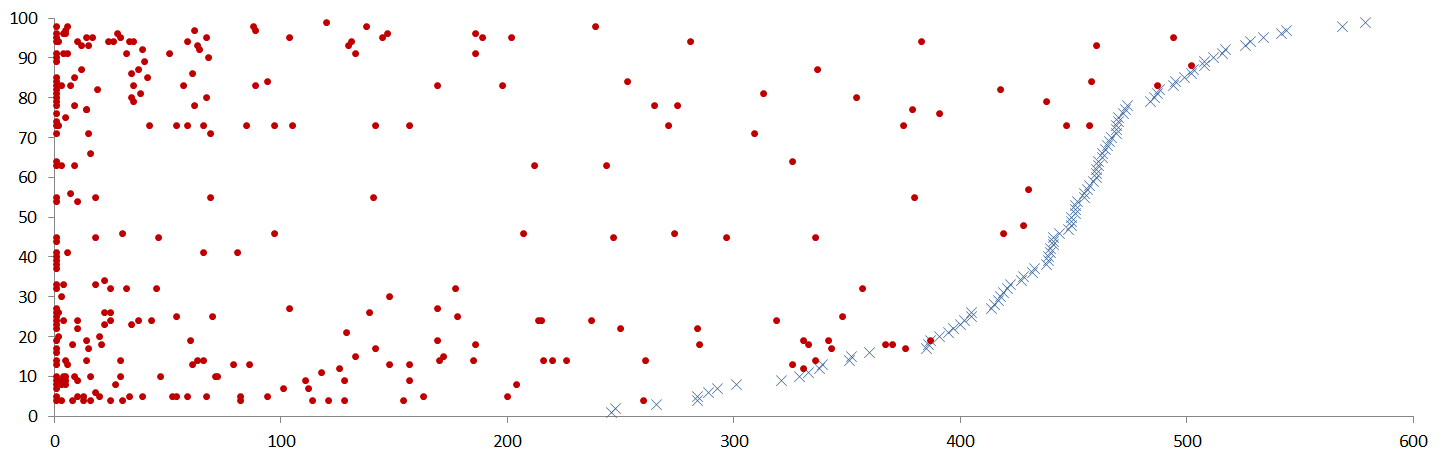
\includegraphics[width=\textwidth]{figures/chapter6/data.png}
\caption{Policy convergence vs. number of revisions}
\label{fig:convergeVSrevisions}
\end{figure}

Figure~\ref{fig:convergeVSrevisions} show all the alarms \st reported in
the experiment.  Each site corresponds to a vertical coordinate in the
figure, and they are sorted according to the total number of requests
executed (due to different ending stage of training phase and stoppage
time between reported alarm and manual inspection, the number of
requests done averages to 434 per site but varies from 246 to 579).
The horizontal axis represents the sequence number of requests, and
alarms are marked along this axis to show when they occurred.  The
majority of alarms are issued at the beginning of the training phase.
The total number of alarms \st reported for all 100 sites is 301 over 40
days, making the average less than three alarms per site per month.  The
highest number of alarms is the 11 alarms reported from \url{mlb.com}.
Of the 100 test sites, 28 issued no alarms at all, which means they do
not need site-specific policies.  Policies of more than half (57) of the
100 sites converge within two policy revisions, and 83 sites converge
within six policy revisions.

\begin{figure}[b]
\centering
\captionsetup{justification=centering}
\includegraphics[width=0.8\textwidth]{figures/chapter6/optimalTrainingOutput}
\caption{Training phase duration vs. Alarm rates}
\label{fig:optimalTrainingOutput}
\end{figure}

\shortsection{Training phase duration} A longer-lasting training phase
observes more behavior but also requires more time and effort.
Figure~\ref{fig:optimalTrainingOutput} shows the relationship between
training phase duration and alarm rates.  Setting the training phase to
conclude after executing 177 requests without an alarm will yield 10\%
of the total alarms.  This number is 20\% for 114 requests, and 70\% for
80 requests.  Based on this, we conclude that \st has observed most
relevant behavior after 200 alarm-free requests and suggest using this
for the convergence threshold after which a learned policy would be
transitions to deployment.

\shortsection{Reasons for alarms}
We manually examined all the alarms.  Violations can be roughly
classified into two general categories, with a few exceptional cases.
The most common reason for a violating record (173 out of 301) is that a
new type of advertisement shows up which was not seen in previous
requests.  For example, \emph{skyscraper} (long and vertical) ads are
only shown on a specific part of the site, whereas other parts show a
\emph{banner} (long and horizontal) ad.  The second category is because
of social network widgets (93 out of 301).  A common scenario is that
news sites serve articles from different sources which do not
necessarily share the same coding pattern and content layout.  This
could result in scripts from \url{twitter.com} injecting Twitter feeds
into containers with different attributes.  Occasionally, the violation
is a result of apparently suspicious behavior or a major script update,
discussed in the next two sections.

\subsection{Suspicious violations}\label{sec:alerting}
In the robustness experiment, we found that on rare occasions the
Facebook scripts load other ad networks and analytics scripts, which
raised massive numbers of alerts.  In some sites such as
\url{staples.com} and \url{dailymotion.com}, Facebook scripts access the
exact same information as did \url{krxd.net} and \url{enlighten.com},
essentially reading the entire page content.  In other cases, Facebook
scripts read the action attribute of all forms on the host page (e.g.,
\url{goodreads.com}, \url{hostgator.com}).  This behavior is only
visible during certain periods of time, and we observed this access on
multiple websites only at the start of the experiment as well as 18 days
after.  In extremely rare occasions (\url{tutsplus.com} and
\url{drupal.org}), \st caught that Facebook scripts read the value of
user's user name and password input on the host page, which is
disturbing.  We are not sure if this is intended by the site owners, and
suspect they are unaware of this behavior.

We have also seen Google advertising scripts read the entire page
contents by calling \code{documentElement.innerHTML}.  This behavior was
only observed once, and only on \url{nfl.com}.  This could be a bug in
an advertising script, or it could indicate that Google advertising is
crawling the page content and indexing it for future contextual
targeting. 

\subsection{Impact of major updates}\label{sec:majorUpdate}

Throughout the course of our evaluation, we saw major changes to three
third-party scripts which resulted in multiple duplicate alarms reported
across most sites embedding them.  Particularly, \url{facebook.net}
scripts began reading properties (e.g. \emph{href}, \emph{rel}) of all
\emph{link} elements on the page since 30 December 2014, and
\url{doubleverify.com} scripts showed similar behavior changes since 5
February 2015.  Additionally, \url{krxd.net} scripts began injecting an
invisible \emph{DIV} element into all pages embedding it since 26
January 2015.  We handled these violations by updating their base
policies since the new behaviors are not site-specific.  These cases
show that while major third-party scripts changes may require updates to
policy, they only occur rarely and trivial changes to base policy are
often enough to cover the new behavior.

It is harder to determine whether a page went through major changes over
our experiment.  However, we did see this for two sites,
\url{theblaze.com}, which added an advertising slot on their frontpage,
and \url{inc.com}, which redesigned its general user interface.  For
both cases, we added an additional advertising container permission to
their site-specific policies.  It can be annoying to the developers to
approve new permissions when a major site update happens, however, we do
not expect policy-breaking changes frequently for most sites.  Further,
we argue that it may be useful to site administrators to learn when a
change impacts the behaviors of scripts significantly enough to require
a policy change.

\section{Prior Works}\label{sec:stRelatedWorks}

\st is directly inspired by our previous work~\cite{Zhou-ESORICS} and intends to improve on some of its limitations, as described in the beginning of this Chapter.  Therefore, we have already covered many related works in Chapter~\ref{sec:esorics_related_works}, including sandboxing JavaScript behavior by extending browsers, rewriting scripts, and encrypting content.  In this section we only focus on comparing \st with previous tools and works that help site administrators understand third-party JavaScript behavior.

\shortsection{Script behavior visualization} Several tools present
script behaviors in a user-understandable way.  Wang et
al.~\cite{Wang:2012:SMY:2310656.2310691} use a browser-based interface
to explore relationships between requests and discover vulnerabilities.
Popular browser extensions like Ghostery~\cite{Ghostery} and
Abine~\cite{Abine} help users and site administrators understand what
third-party services exist on the current page.  A recent Chrome
developer tool~\cite{ChromeDeveloperTool} informs a user what resource a
Chrome extension is accessing on the page, albeit at coarse granularity.
The success of these tools supports our hope that our tool chain can be of
great value to web developers in understanding scripts and developing
policies.

\section{Deployment}\label{sec:stDeployment}

In this section, we discuss some possible deployment scenarios.  So far,
we have focused on the scenario where a site administrator wants to
understand the behaviors of embedded scripts on a web site to protect
clients from privacy compromises by malicious or compromised scripts and
ensure the integrity of the site from unintended modifications.  The
tools we developed could be used in several other ways, discussed below.

\shortsection{Access visualization} \vis can be used by either an
interested web developer or sophisticated user.  After examining the
accessed resources, a developer can make an informed decision to choose
the service provider that most respects site integrity and user privacy.
A sophisticated user may use extensions like noscript~\cite{noscript} to
block third-party scripts with suspicious behaviors revealed by \vis.

\shortsection{Policy generation service} A third-party service provider
or dedicated security service could develop base policies for
commonly-used scripts.  A cooperating third-party service provider may
make site-specific policy generation part of the implementation process.
For example, policies can be inferred by analyzing the implementation
code.  In a less ideal scenario, the policy generation service could
provide a description of how to generate a site-specific policy for the
script based on properties of the embedding site.  Site administrators
would then use that description to manually generate their own
site-specific policies.

\shortsection{Access monitoring} After a policy has been generated, we
envision two ways a site administrator can monitor future accesses.  An
easy-to-adopt approach is to continue running \st with the policies on
simulated sessions.  An alternative approach is to sample real world
traffic using a reverse proxy and forward sampled requests to run in \st
with user credentials.  The second approach gives higher confidence that
the integrity and privacy properties are not violated in real sessions,
but risks interfering with the normal behavior of the site if repeating
requests alters server state.  For both cases, the site administrator
would examine alerts and respond by either changing policies or altering
the site to remove misbehaving scripts.  More security-focused sites
could automate this process to automatically remove scripts that
generate alarms.

\shortsection{Policy enforcement}\label{sec:enforcement} Our prototype
\st is not intended to be used by end users to enforce the policies at
runtime mainly due to its high runtime overhead.  The key reason is that
each DOM API access requires at least one stack computation and node
removal APIs require walking the subtree and compute access violations.
However, some policies may be enforced by other browser security
mechanisms, for example, scripts from a particular domain can be
blacklisted by content security policy, which is currently supported by
major browsers.  We envision a future, though, where a more expressive
analog to CSP is adopted by popular browsers and servers can provide
headers with restrictive policies for embedded scripts that would be
enforced by browsers at runtime.  This would offer the best protection,
ensuring that the actual behavior of the dynamically-loaded script on
client's browser does not behave in ways that violate the server's
script policy.
